\section{Endogenous Pension Design}\label{sec:esc}
Throughout the paper so far the Bismarckian index $\theta$ is calibrated and held fixed while taxes are chosen politically. This section endogenizes the relation between contributions and benefits. The design is chosen by the same probabilistic-voting objective $\mathcal{W}_t$ that sets $\tau_t$, in the model without informal households. We explore four variants, three related to the \emph{timing} of the choice (made contemporaneously, one period in advance, or once and for all), and a \emph{deadweight cost} of the redistribution that flat benefits perform. We find that with costless redistribution all three timings put the design at a corner: the Beveridgean corner, $\theta = 0$, at observed U.S.\ inequality, except for the permanent choice at high intertemporal elasticities, where it is the Bismarckian one. An interior choice requires redistribution through the pension system to be costly. Our preferred specification is therefore the choice \emph{one period in advance with a deadweight cost that scales with the redistribution performed and with the size of the system}, calibrated so that the 2020 electorate re-elects the system it has. Under this specification ageing makes the chosen design more Bismarckian, since a larger system makes flat benefits costlier to keep, France's voting profile makes it less so, increasingly with the intertemporal elasticity, and France's income distribution leaves it interior at every elasticity and moves it less than voting patterns do. The cost is calibrated on one datum, the U.S.\ design, and the same parameter orders the designs of the UK, the U.S.\ and France as observed. This section states the four variants, the argument for the preferred one, and the results; derivations, algorithms and the full verification battery are in the online technical documentation published alongside the paper.\footnote{\textcite{BergGE26doc}, section \textit{Endogenous system characteristics}. It contains the model definitions and propositions for each timing, the derivation of the cost, the numerical algorithms (including the exact two-dimensional policy-function recursion under CRRA and the checks behind every structural claim used here), and the calibration protocol.}

\subsection{Three timings, one corner}
\smalltitle{Contemporaneous.} If $\theta_t$ is chosen at $t$ together with $\tau_t$, it only re-splits benefits already granted. Current labor supply depends on the \emph{next} period's choice, $\theta_{t+1}$, so there is no strategic channel, and the marginal effect on the political objective runs entirely through current retirees,
\begin{align}\label{eq:esc:seqFOC}
   \dfrac{\partial \mathcal{W}_t}{\partial \theta_t} =\omega \sum_i\gamma_i\mu_i\frac{\frac{1-\alpha}{\alpha}\tau_t\left(\frac{\eta_{i}^{1+\xi}}{X_{i}^{\xi}}\frac{1}{\Gamma_{h}}-1\right)}{\frac{s_{t-1}^i}{s_{t-1}}+\frac{1-\alpha}{\alpha}\tau_t\left(1+\theta_t\left[\frac{\eta_{i}^{1+\xi}}{X_{i}^{\xi}}\frac{1}{\Gamma_{h}}-1\right]\right)}\;\leq\;0 \quad\text{for } \theta_t\in[0,1].
\end{align}
With equal voting weights the numerator would average to zero across types and the sign would be the denominator's, which is larger for high-income retirees. The voting weights $\mu_i$ rise with income, so the sign is a quantitative matter. Evaluated at the calibrated 2020 equilibrium the expression is negative over the whole interval $[0,1]$, at every date of the projection and at $\rho = 0.5$, $1$ and $2$: lowering $\theta_t$ redistributes from retirees with low marginal utility to retirees with high marginal utility, and the choice is the corner $\theta = 0$.

\smalltitle{Advance.} If instead $\theta_{t+1}$ is chosen at $t$, the design becomes a state variable with forward-looking content: it moves current labor supply and savings both directly (the economic-equilibrium effect) and through the anticipated response of $\tau_{t+1}$ (the politico-economic effect), and it no longer touches the benefits of current retirees. With the political objective of \eqref{eq:LOG:PolObj}, the marginal effect is
\begin{align}\label{eq:esc:leadFOC}
   \dfrac{\partial \mathcal{W}_t}{\partial \theta_{t+1}} = \sum_i\gamma_i\mu_i\left[\omega\,(1-\alpha)\dfrac{d\ln\Theta_{h,t}}{d\theta_{t+1}} + \nu_t\left((1+\beta)\dfrac{d\ln\tilde{c}_{1,t}^i}{d\theta_{t+1}} + \beta\dfrac{d\ln R_{t+1}}{d\theta_{t+1}}\right)\right],
\end{align}
where $\Theta_{h,t}$ is the labor supply function of appendix \ref{app:EE:LOG} and each total derivative includes the response of $\tau_{t+1}$, and of $\theta_{t+2}$, to the design being chosen. Retirees are unanimous, since their term does not depend on $i$, and they favour a more contributive system: a higher $\theta_{t+1}$ raises the return to an hour worked at $t$ and with it the labor supply on which their benefits are levied. The young are divided, and the sign of the sum is a quantitative matter. The equilibrium is a sequence of policy functions over the inherited design, identified by backward induction as in section \ref{sec:numerical}. The redistributive force of \eqref{eq:esc:seqFOC}, now operating through the young's own future benefits, nonetheless dominates, and at observed U.S.\ inequality the choice is again the corner $\theta = 0$ for reasonable labor supply elasticities.

\smalltitle{Permanent.} If a design chosen at $t_0$ is expected to hold forever, it enters all channels at once: the re-splitting of current benefits in \eqref{eq:esc:seqFOC}, the labor-supply channel of \eqref{eq:esc:leadFOC}, and the whole continuation path of taxes. The outcome is again a corner. Under log preferences it is $\theta = 0$; under CRRA the forward-looking channels grow with the elasticity, and for $\rho$ above about $1.3$ the corner is the Bismarckian one, $\theta = 1$. On either side of that switch the electorate is close to indifferent between the two corners, so the elasticity at which it occurs is not sharply located; what does not depend on the elasticity is that the choice is a corner.\footnote{The joint choice of $\tau_{t_0}$ and $\theta$ reduces to a one-dimensional search, since the tax condition at any candidate design is the ordinary one, and the savings the electorate takes as given are those of households who anticipated the vote; the technical documentation gives the algorithm and its checks. The model with a permanent choice of $\theta$ can be calibrated to the observed 2020 characteristics only under counterfactually compressed inequality.}

The common lesson is that in this class of models a costless choice never lands in the interior: some friction must make Beveridgean pensions more expensive than Bismarckian ones for an interior design to survive.

\subsection{Costly redistribution, and the preferred specification}
We introduce a deadweight cost of the redistribution that the flat component of benefits performs, so that the government budget becomes
\begin{align}\label{eq:esc:budget}
    \nu_t w_t\tau_th_t\, f(\theta_t,\tau_t) &= \sum_i \gamma_i b_t^i, \\
    f(\theta_t,\tau_t) &= \exp\!\left(-\tfrac{1}{2}\,\lambda\,\tau_t\,\tilde{V}\,(1-\theta_t)^2\right), \qquad \tilde{V} \equiv \sum_i\gamma_i\frac{(y_i-1)^2}{y_i}, \qquad y_i \equiv \frac{\eta_i^{1+\xi}}{X_i^{\xi}\,\Gamma_h}, \nonumber
\end{align}
where $y_i$ is the labor income of type $i$ relative to the mean, $\lambda \geq 0$ is the cost parameter, and a share $1-f$ of revenue does not reach retirees. The cost has three arguments: the share of the benefit that is flat, $1-\theta_t$, the dispersion of relative incomes, $\tilde{V}$, and the size of the system, $\tau_t$. Nothing is lost when nothing is redistributed: $f = 1$ at $\theta_t = 1$, and $f = 1$ for every design when all incomes are equal, where a flat and an earnings-related benefit pay the same to everyone.

The form follows from reading the flat component as a tax. Part of a pension contribution buys the contributor a benefit and part does not, and only the second part distorts like a tax. This is the tax component of contributions of \textcite{Summers89a1}. The model already contains the hours response to it, since the contributive share of next period's benefit raises the return to an hour worked and hours respond through the Frisch elasticity. The cost stands for the margins the model does not contain, and the evidence finds the tax component to matter on two of them. \textcite{Disney04a1} splits pension contributions in OECD countries into a tax and a saving component and finds that the tax component lowers the labor force participation of women, while the saving component raises it. \textcite{KumlerVF20a1} find that when Mexico's 1997 reform tied pension benefits more closely to reported wages, the underreporting of wages to the social security agency fell for the workers affected. On a participation or a reporting margin the wedge that matters is the average tax on the earnings at stake rather than the marginal one \parencite{Saez02a1,KlevenK06a1}, and the average implicit tax of the flat component differs across types. Relative to a purely earnings-related system paying the same revenue, the flat component moves the benefit of type $i$ by $\tau_t(1-\theta_t)(1/y_i-1)$ per unit of past earnings: a tax on types above mean income, a subsidy to types below it, and a pure transfer in the aggregate.\footnote{Up to the pay-as-you-go return factor $\Pi_t = \nu_t w_t h_t/(w_{t-1}h_{t-1})$, which multiplies every implicit tax alike and which we absorb into $\lambda$, so that an elasticity $\varepsilon$ corresponds to $\lambda = \Pi_t\varepsilon$. The factor is of the order of $\nu_t$, which is $1.34$ for the U.S.\ in 2020. The technical documentation gives the derivation.} The deadweight loss of a set of such wedges is the sum of their \textcite{Harberger64a1} triangles, and with a common elasticity $\varepsilon$ it is $\tfrac12\varepsilon\,\tau_t(1-\theta_t)^2\tilde{V}$ as a share of revenue, which is $1-f$ in \eqref{eq:esc:budget} to first order with $\lambda$ in the place of $\varepsilon$.\footnote{The quadratic counts the subsidy to types below mean income as a loss, as it does the tax on types above it. Where participation is already taxed, lowering the participation tax of low-income workers can reduce the total loss \parencite{Saez02a1}, so the symmetry is a property of the reduced form rather than of the argument.}

Each argument of $f$ is a consequence of this reading. The loss is quadratic in the flat share $1-\theta_t$ because it is quadratic in each wedge. It is proportional to $\tilde{V}$ because the wedges scale with the distance of relative incomes from the mean, so a compressed income distribution lowers the redistribution a flat benefit performs and the cost of performing it together. And the loss per unit of revenue is linear in $\tau_t$, since the loss rises with the square of the implicit tax while revenue rises with the tax itself. The last property links the size of the system to its design. It is the efficiency--redistribution trade-off by which \textcite{KoethenbuergerPP08a1} account for the finding of \textcite{CondeRuizP07a1} that more redistributive systems are smaller, here read from the other side: a larger system is costlier to keep redistributive. The shape of $f$ thus follows from the tax component, but its size does not. At $\rho \leq 1$ the calibrated $\lambda$ (table \ref{table:US_ESC:calibration}) is more than an order of magnitude above what participation and taxable-income elasticities of $0.1$ to $0.4$ would give \parencite{ChettyGMW11a1,SaezSG12a1}, and at $\rho = 2$ it is roughly three to thirteen times as large, so $\lambda$ also stands in for administrative, evasion and political costs of redistribution that the model does not contain.\footnote{The cost is proportional, scaling both components of the benefit alike. The alternative attaches it to the flat component only; it delivers the same endpoints and differs in the interior, at a cost in identification, since $f$ then no longer cancels from the replacement-rate ratio and $\theta^{\ast}$ and $\lambda$ are identified jointly. A cost attached to the design itself rather than to the transfer it performs, $f(\theta) = \phi + (1-\phi)\theta^{p}$, was the specification of an earlier draft; appendix \ref{app:US:escTables} reports it as a robustness check.}

With the cost, the benefit formula carries $A(\theta_t,\tau_t) = f(\theta_t,\tau_t)\,\theta_t$ and $B(\theta_t,\tau_t) = f(\theta_t,\tau_t)\,(1-\theta_t)$ in place of $\theta_t$ and $1-\theta_t$. The design enters the economic equilibrium only through these two groups, so the cost is exactly that substitution in the equilibrium functions ($\Gamma_{s}$, $\Theta_{h}$, relative savings). Because the cost is proportional, it also cancels from the replacement-rate ratio that identifies $\theta$ from the OECD data, and the data target is unchanged, $\theta^{\ast} = 0.738$. In the tax condition the cost adds one factor. Since $f$ falls with the tax that funds it, the benefit term of the retirees' marginal effect $\mathcal{E}_{2,t}^i$ in appendix \ref{app:PEE:LOG} is multiplied by $1+\tau_t\,\partial_{\tau}\ln f = 1+\ln f(\theta_t,\tau_t)$, so a larger system is worth less to a retiree at the margin than the revenue it collects.

We let the design be chosen one period in advance, and use only this timing with the cost, for three reasons. First, a design chosen for the current period only re-splits benefits that current retirees have already earned. It moves no labor supply or savings decision, so the cost would be the only force against the Beveridgean corner of \eqref{eq:esc:seqFOC}, and the design would be a pure transfer among retirees. Second, a design chosen once and for all requires commitment expectations that are difficult to reconcile with the Markov equilibria of the rest of the paper. Third, the choice one period in advance keeps the Markov structure and is the only timing in which the design affects current labor supply and savings before it binds, which is the channel through which $\theta$ moves taxes and savings in section \ref{sec:oecd}. It also mirrors how reforms of benefit formulas are commonly legislated, applying to future benefits and leaving benefits in payment untouched.

In this timing the design in force, $\theta_t$, is a state: its cost $f(\theta_t,\tau_t)$ enters only the benefits of current retirees and, through them, the tax condition above. The design chosen at $t$, $\theta_{t+1}$, enters the condition \eqref{eq:esc:leadFOC} through next period's groups $A(\theta_{t+1},\tau_{t+1})$ and $B(\theta_{t+1},\tau_{t+1})$, with $\tau_{t+1}$ the anticipated equilibrium tax. In the labor supply function,
\begin{align}\label{eq:esc:leadFOCcost}
   \dfrac{d\ln\Theta_{h,t}}{d\theta_{t+1}} = \frac{\xi}{1+\alpha\xi}\;\frac{\frac{1-\alpha}{\alpha}\,\dfrac{d}{d\theta_{t+1}}\!\left[A(\theta_{t+1},\tau_{t+1})\,\tau_{t+1}\,\Gamma_{s,t}\right]}{\Gamma_{h}-\frac{1-\alpha}{\alpha}A(\theta_{t+1},\tau_{t+1})\,\tau_{t+1}\,\Gamma_{s,t}},
\end{align}
so that the return to an hour worked at $t$ rises with the contributive share $A(\theta_{t+1},\tau_{t+1})$ of next period's benefit, net of the anticipated tax response and of the response of $\Gamma_{s,t}$, which carries $A$ and $B$ as well. What makes an interior choice possible is how the two groups move with the design. At a given tax, $\partial_{\theta}A = f + \theta_{t+1}f_{\theta}$ and $\partial_{\theta}B = (1-\theta_{t+1})f_{\theta} - f$, where $f_{\theta} = f\,\lambda\tau_{t+1}\tilde{V}(1-\theta_{t+1})$. Without the cost a more Bismarckian design shifts next period's benefits one for one from the flat to the earnings-related component, $\partial_{\theta}A = -\partial_{\theta}B = 1$, and the redistributive stake of the young dominates, as in the previous subsection. With the cost $\partial_{\theta}A + \partial_{\theta}B = f_{\theta} \geq 0$: a more Bismarckian design also raises the total the young will receive, since it dissipates less. This gain is zero at $\theta_{t+1} = 1$ and rises with the flat share, the dispersion of incomes and the size of the system the young anticipate, so the design condition can cross zero in the interior. The anticipated tax response carries the cost as well, since $f$ falls with $\tau_{t+1}$. The explicit expressions are in the technical documentation, together with the proofs that the substitution, the independence of the tax from next period's policy and, under log preferences, the independence of the chosen design from the inherited state all survive the cost.

\subsection{Results}
\smalltitle{Calibration.} The cost parameter is identified separately from the design, by requiring that the design in force in the calibration year, on a path where the political choice binds from the first period, is the observed one,
\begin{align}\label{eq:esc:calibration}
    \theta_{t_0} = \Theta_{t_0-1}\!\left(\theta^{\ast}\right) = \theta^{\ast},
\end{align}
with $(\beta,\omega)$ recalibrated at every trial value of $\lambda$. The calibration pins the design in the calibration year only. The design chosen at every later date is a prediction of the model, and the results below report how it drifts as population growth slows along the projected path.

Table \ref{table:US_ESC:calibration} reports the calibrated cost across the paper's range of intertemporal elasticities, at the U.S.\ dispersion of relative incomes $\tilde{V} = 0.436$. The cost required for the electorate to re-elect the observed design falls in $\rho$ by a factor of about ten: $\lambda = 18.242$, $8.643$ and $1.728$ at $\rho = 0.5, 1, 2$. At those values the observed design loses $3.9\%$, $1.8\%$ and $0.4\%$ of revenue at the 2020 size of the system ($f(\theta^{\ast},\tau_{2020}) = 0.961$, $0.982$ and $0.996$), and a fully flat system of the same size would lose $44\%$, $24\%$ and $5\%$. The reason for this is that a higher elasticity strengthens the forward-looking (savings and labor supply) channels in a Bismarckian system, so less friction is needed to hold the choice away from the Beveridgean corner. We view this, together with the effect of $\rho$ on savings after pensions became universal in Argentina (section \ref{sec:argentina}) and with the calibrated cost lying closest to estimated elasticities at $\rho = 2$, as further evidence that calibrations with $\rho \in [1,2]$ are more empirically plausible.

%% GENERATED by python/paper/build.py from results/ -- do not edit by hand.
%% Rebuild:  .venv\Scripts\python.exe python\paper\build.py --only US_ESC_Calibration
%% Source:   results/esc/escCalibration{,CRRA}.csv
\begin{table}[!htb]
\centering
\begin{threeparttable}
\caption{The calibrated cost of redistributive funds}
\label{table:US_ESC:calibration}
\renewcommand{\arraystretch}{1.25}
\begin{tabularx}{.9\textwidth}{YYYY}
\toprule
\textbf{CRRA} ($\rho$) & $p$ & $\theta^{\ast}$ & $f(\theta^{\ast})$ \\
\midrule 
0.5 & 0.935 & 0.738 & 0.876 \\
1.0 & 0.408 & 0.738 & 0.942 \\
2.0 & 0.085 & 0.738 & 0.987 \\
\bottomrule
\end{tabularx}
\begin{tablenotes}[flushleft]
\footnotesize
\item[] \textit{Note:} $f(\theta) = \phi + (1-\phi)\theta^{p}$ with $\phi = 0.5$ imposed; $p$ is calibrated so the $\theta$ choice is the observed one, with $(\beta, \omega)$ recalibrated at each trial value. The cost is proportional, so the wedge cancels from the replacement-rate ratio. Without the cost the choice would be in the corner $\theta = 0$ for every $\rho$.
\end{tablenotes}
\end{threeparttable}
\end{table}


\smalltitle{Solution.} For $\rho = 1$ the equilibrium with the design chosen one period in advance is solved exactly. Under log preferences the model without informal households carries no endogenous state (section \ref{sec:numerical}), so the equilibrium tax at any date, given the designs in force, is a scalar problem in $\tau_t$ alone, and the design chosen at $t$ is provably independent of both the savings state and the design inherited. Each date's choice is therefore a one-dimensional search over the design grid, with no state to carry. Under CRRA neither property survives, and the equilibrium is a backward recursion over policy functions on the two-dimensional state $(s_{t-1},\theta_t)$: at each date, for every inherited savings level and design and for every candidate design, the equilibrium tax and the continuation are resolved, and the candidate that maximizes the objective is selected. The objective is flat near its maximum, so the chosen design is reported to the resolution of the candidate grid. Details and the verification battery are in the technical documentation.

\smalltitle{Baseline path.} By construction the design in force in 2020 is $\theta^{\ast}$ at every $\rho$. Along the baseline demographic path the chosen design then drifts Bismarckian as ageing proceeds: at $\rho = 1$ from $0.738$ in 2020 to $0.797$ by 2050, $0.804$ by 2080 and $0.809$ from 2110 on, tracking the projected fall in $\nu_t$ and flattening when it does, and to $0.798$ and $0.817$ by 2110 at $\rho = 0.5$ and $2$. At $\rho = 1$ the tax rate rises from $14.4\%$ to $19.5\%$, $20.9\%$ and $20.9\%$ along the same path, between $0.1$ and $0.2$ p.p.\ above the path with the design held at $0.738$, since a more Bismarckian system dissipates less and is worth more to the electorate at the margin. Each counterfactual below is a separate equilibrium \emph{path}: the changed characteristic holds over the whole horizon, the economy starts from its own steady state, and the political choice binds from the first period. A row therefore describes a country that has always had this mix of characteristics rather than the U.S.\ surprised in 2020, which makes it comparable with France's own calibrated path. Because the choice binds from the first period, the design in force in 2020 is itself an equilibrium outcome rather than an inherited datum, and every row is read at 2020. The tables in appendices \ref{app:US:escTables} and \ref{app:US:ukESC} compare, for each counterfactual, the shocked economy with the design \emph{pinned} at the observed U.S.\ value (exogenous $\theta$) and with the design \emph{chosen} (endogenous $\theta$), at $\rho \in \{0.5, 1, 2\}$. Both readings carry the cost and start from the same design, $\theta = 0.738$, so the distance between them is the political response to the changed characteristic.\footnote{We report the chosen design under the common-$X$ calibration of section \ref{sec:oecd} only. The design enters the political objective only through the relative incomes $y_i$ of \eqref{eq:esc:seqFOC}, which both calibrations match to the same data, and the same is true of the cost, whose $\tilde{V}$ is a function of relative incomes alone; the two calibrations share $\beta$, $\omega$, the tax rate and the savings rate, so the ageing and voting counterfactuals do not turn on the choice. The income-distribution counterfactual and the composite that contains it are defined through $\eta$ and $X$ separately and do: in the exogenous-design model of section \ref{sec:oecd}, France's distribution lowers the tax rate by 1.6 p.p.\ under the vector-$X_i$ calibration of appendix \ref{app:US:vectorX} against 1.2 p.p.\ under the common-$X$ one, so the design response reported below for those two rows would be read against a larger exogenous change.}

Figure \ref{fig:US_ESC:overview} collects the whole set. For every counterfactual and every $\rho$, an open marker is the reading with the design pinned at the U.S.\ value and a filled marker the reading with the design chosen, joined by a connector, so the length of each connector is what endogenizing the design adds. The first panel shows the design itself as a level: every pinned marker sits at $0.738$ by construction, and the connector is the political response. The tax, savings and workweek panels are deviations from the baseline, and a connector that collapses to a single dot marks a counterfactual whose design response leaves that variable essentially unchanged. At $\rho \leq 1$ the design response moves hours by at most $0.1$ hours a week in every counterfactual, so the hours effect of a counterfactual is its exogenous one. At $\rho = 2$ the design moves far enough under French voting to cost about half an hour a week, $38.6$ against $39.1$ hours with the design pinned (table \ref{table:US_ESC:voting}), and about $0.4$ hours under the composite of French characteristics, while acute ageing adds $0.1$ hours.

\begin{figure}[!htb]
    \centering
    \caption{Endogenous versus exogenous pension design across counterfactuals}
    \label{fig:US_ESC:overview}
\begin{threeparttable}
    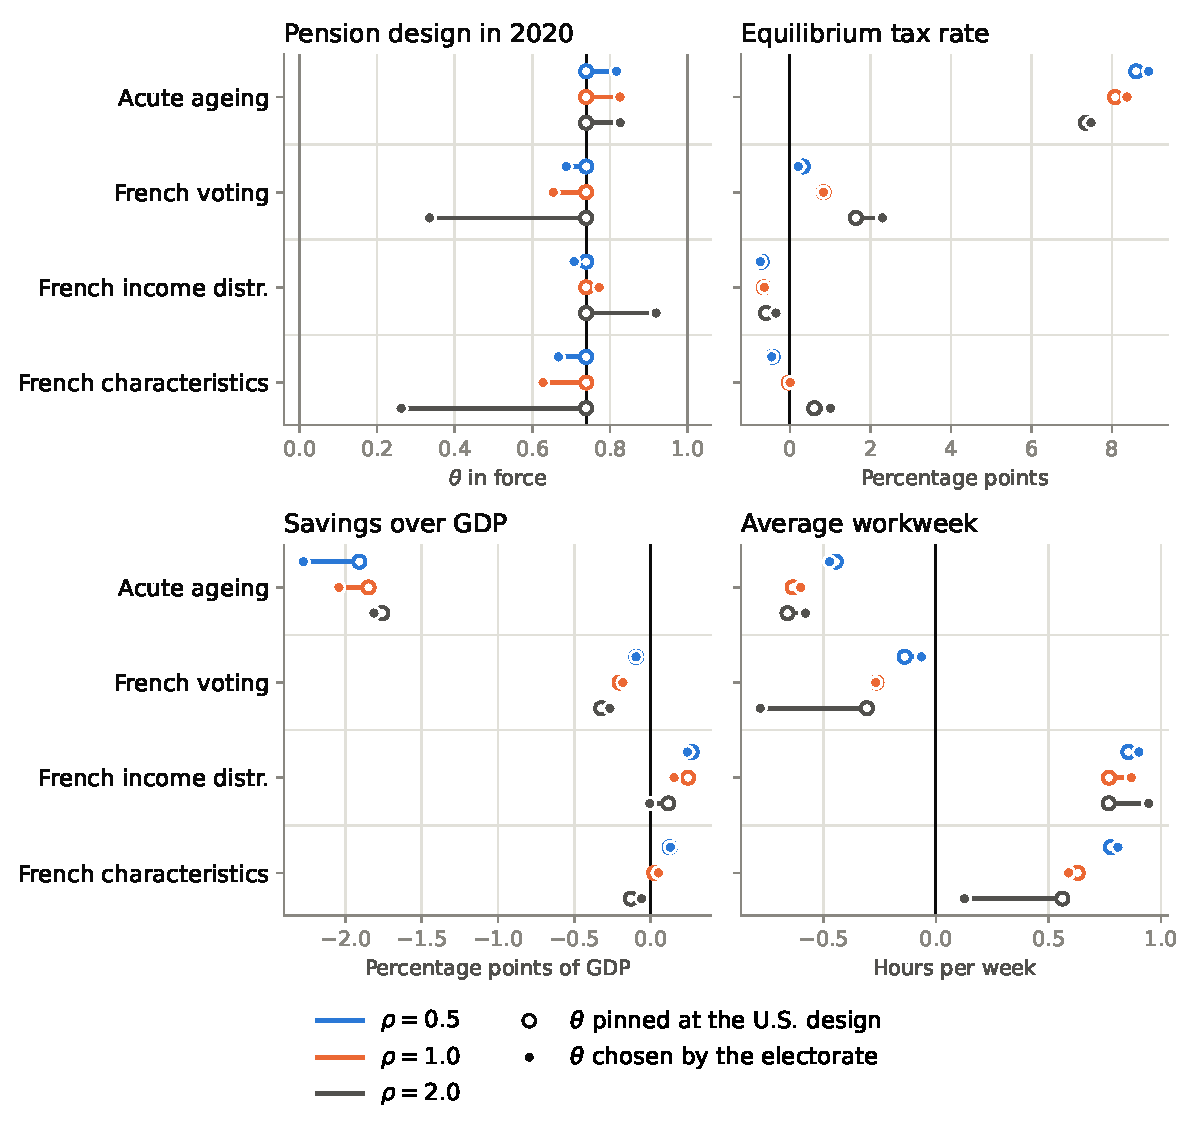
\includegraphics[width=\linewidth]{Figs/US_ESC_overview.pdf}
\begin{tablenotes}[flushleft]\footnotesize
    \item[] \textit{Note:} The first panel is the design in force as a level, with the muted lines at the corners $\theta = 0$ and $\theta = 1$; the other three are deviations from the endogenous-$\theta$ baseline, whose levels are the baseline rows of table \ref{table:US_ESC:ageing}. The savings rate is savings relative to GDP.
\end{tablenotes}
\end{threeparttable}
\end{figure}

\smalltitle{Ageing.} Acute ageing ($\nu_t = 1$ throughout) raises the chosen design at every elasticity, from $0.738$ to $0.817$, $0.825$ and $0.826$ at $\rho = 0.5, 1, 2$, and mild ageing raises it to $0.784$ at $\rho = 1$ (table \ref{table:US_ESC:ageing} in appendix \ref{app:US:escTables}). The response varies little with the elasticity, unlike the calibrated cost. Two mechanisms add up. A scarcer young generation raises the political weight of retirees, who are unanimous for a more contributive system in \eqref{eq:esc:leadFOC}; and the tax that ageing calls for makes the flat component costlier at the margin, since the loss in \eqref{eq:esc:budget} is proportional to $\tau_t$. Under acute ageing the tax rises from $14.4\%$ to $22.8\%$, so the loss per unit of redistribution rises by more than half, and this second channel is what makes the response first order. The tax and savings responses themselves are essentially those of the exogenous-$\theta$ reading: at $\rho = 1$ the chosen design adds $0.3$ p.p.\ to a tax response of $8.1$ p.p.\ under acute ageing and $0.1$ p.p.\ to the $3.7$ p.p.\ of mild ageing, since a more Bismarckian system dissipates less and is therefore worth a larger tax to the electorate. The difference is $0.3$ p.p.\ at $\rho = 0.5$ as well ($23.3\%$ against $23.0\%$) and $0.1$ p.p.\ at $\rho = 2$ ($21.9\%$ against $21.8\%$), where the cost is thin. The pinned reading responds a little less than in section \ref{sec:oecd}, $8.1$ against $8.7$ p.p., because with the cost in place a larger system is worth less to retirees at the margin. A small part of the fiscal adjustment thus runs through the system's shape rather than its size, in the direction of earnings-related benefits.

\smalltitle{Income distribution.} Holding $\theta$ at the U.S.\ value, France's flatter income distribution lowers the equilibrium tax at $\rho = 1$ from $14.4\%$ to $13.8\%$ and raises savings (table \ref{table:US_ESC:incomeDistr}). The fall is smaller than the $1.2$ p.p.\ of section \ref{sec:oecd} because a compressed distribution also lowers $\tilde{V}$, and with it the share of revenue the flat component dissipates, so the system is worth more at the margin. When the electorate chooses the design it moves to $0.772$, an interior response of the same order as mild ageing. This happens because the cost in \eqref{eq:esc:budget} is proportional to the same dispersion of relative incomes as the redistribution a flat benefit performs: compressing the distribution lowers the redistributive stakes and the cost of carrying them together, and what remains is a small net effect whose sign depends on the elasticity. The chosen design is $0.708$ at $\rho = 0.5$, below the U.S.\ value, and $0.919$ at $\rho = 2$, interior at every elasticity and rising in it, since a higher elasticity strengthens the young's forward-looking stake in earnings-related benefits, which does not scale with the dispersion of incomes and so gains ground when the redistributive stakes shrink. The design response leaves the tax essentially where the pinned reading puts it, $13.8\%$ in both readings at $\rho = 1$ and $13.7\%$ at $\rho = 0.5$, and adds $0.2$ p.p.\ at $\rho = 2$, $14.1\%$ against $13.8\%$; savings move by less than $0.2$ p.p.\ of GDP. The model therefore does not tie the design tightly to inequality: the response is interior at every elasticity and small at $\rho \leq 1$, in line with the weak relation between inequality and the Bismarckian index across countries in figure \ref{fig:US:OECDdata}.

\smalltitle{Voting patterns.} France's much flatter voting-weight profile pushes the design toward the Beveridgean corner, and this is the experiment whose strength depends most on the elasticity: the chosen design falls from $0.738$ to $0.687$ at $\rho = 0.5$, $0.653$ at $\rho = 1$ and $0.334$ at $\rho = 2$ (table \ref{table:US_ESC:voting}). When the poor carry more relative voting weight, the redistributive force of \eqref{eq:esc:seqFOC} regains ground against the forward-looking stake; at $\rho = 1$ the response is of the same size as that of acute ageing, with the opposite sign. That the design falls furthest at the highest elasticity, where that stake is strongest, is a consequence of the calibration: the cost is set to re-elect the observed design at each $\rho$, and it takes only $0.4\%$ of revenue at $\rho = 2$ against $3.9\%$ at $\rho = 0.5$ (table \ref{table:US_ESC:calibration}), so at a high elasticity the interior choice is held in place by a thin cushion and a stronger redistributive pull moves it a long way. In the exogenous reading a flatter voting profile makes the system larger, by $0.8$ p.p.\ at $\rho = 1$. At $\rho \leq 1$ the design response leaves that tax essentially where it is, $15.3\%$ in both readings at $\rho = 1$, because the less Bismarckian design chosen also dissipates more revenue, which offsets the usual pull of a flatter benefit toward a larger system; at $\rho = 2$, where the design moves a long way and the cost is thin, the tax ends above the pinned reading, $16.7\%$ against $16.1\%$.

\smalltitle{Both at once.} When France's income distribution and voting profile are imposed together, the two forces pull the design in opposite directions and the voting profile prevails at every elasticity: the chosen design is $0.667$, $0.627$ and $0.261$ at $\rho = 0.5, 1, 2$, below the U.S.\ value throughout and increasingly so as the elasticity rises, with the tax at $14.4\%$ in both readings at $\rho = 1$ and $15.4\%$ against $15.0\%$ at $\rho = 2$. Adding France's level of $X_i$ on top, so that the U.S.\ carries all of France's household characteristics (table \ref{table:US_ESC:frenchAll}), changes none of this. A common rescaling of $X_i$ moves hours and nothing else, since aggregate hours carry no scale of their own (section \ref{sec:oecd}), so those rows carry the same design and tax as the pair and differ only in hours; on its own, France's level of $X_i$ leaves the chosen design at $0.738$ at every elasticity, to the resolution of the candidate grid, which is the placebo the construction implies. The model therefore signs the effect of French household characteristics on the design: they make it less Bismarckian at every elasticity, the voting profile outweighing the compressed income distribution, and the size of the effect grows with $\rho$. What the characteristics do not deliver is France's own design, the corner $\theta = 1$, which we take up next.

\smalltitle{Across countries.} The cost is calibrated on one datum, the U.S.\ design, so the UK and France are a test of the specification rather than of its fit. Table \ref{table:US_ESC:country} (appendix \ref{app:US:ukESC}) lets each electorate choose the design on its own calibrated path under the U.S.\ parameter $\lambda = 8.643$, at $\rho = 1$. The UK, with an observed design of $0.560$ and a tax rate of $11.9\%$, chooses $0.625$; France, with the corner $\theta = 1$ and $21.3\%$, chooses $0.749$; the U.S.\ re-elects $0.738$ by construction. The observed ranking of the three, the UK below the U.S.\ below France, is thus reproduced from one parameter, though compressed. The reason for this is the size of the system: the UK and France have nearly the same dispersion of relative incomes at the U.S.\ income cuts, $\tilde{V} = 0.223$ and $0.218$, both about half the U.S.\ value, and what separates their chosen designs is the tax that funds them, $11.9\%$ against $21.3\%$, which is the relation between the size of the system and its design that figure \ref{fig:US:OECDdata} shows. Calibrating the UK's own cost, so that its electorate re-elects $0.560$, gives $\lambda = 7.264$, within $16\%$ of the U.S.\ value; regrouping the UK at the U.S.\ income percentiles, which lowers its $\tilde{V}$ to $0.065$, moves the choice under the U.S.\ parameter only from $0.625$ to $0.644$, so the result does not turn on how the income groups are cut. France has no own cost: its observed design is the corner, and under a cost quadratic in the redistribution performed the first unit of redistribution is free at the margin, so no electorate chooses exactly $\theta = 1$ and no finite $\lambda$ reproduces France's design. A linear term in $1-\theta$ would restore that possibility at the price of a second parameter, which the UK's design could pin with France as the prediction; we leave it for future work. The cost parameter absorbs whatever makes redistribution through pensions expensive, and the cross-country test is what disciplines it: one value calibrated on the U.S.\ orders the three designs and comes within $16\%$ of the UK's own, while the corner France occupies lies outside what a purely quadratic cost can deliver.
